% =============================================================
% บทที่ 3 - วิธีดำเนินงานโครงงาน
% =============================================================

ในการดำเนินโครงงาน "การวิเคราะห์และทำนายผลการแข่งขันฟุตบอลพรีเมียร์ลีกอังกฤษด้วยกระบวนการวิทยาการข้อมูล (English Premier League Match Analysis and Prediction Using Data Science Process)" ผู้จัดทำได้กำหนดขั้นตอนการดำเนินงานตามกระบวนการวิทยาการข้อมูล (Data Science Pipeline) เพื่อให้การวิเคราะห์และการพัฒนาแบบจำลองมีความเป็นระบบ แม่นยำ และสามารถตรวจสอบซ้ำได้ โดยแบ่งขั้นตอนการดำเนินงานออกเป็น 5 ส่วนหลัก ดังนี้

\begin{enumerate}[label=\arabic*)]
    \item การวิเคราะห์และกำหนดแนวทางการพัฒนาโครงงาน
    \item การเก็บรวบรวมและเตรียมข้อมูล (Data Collection \& Preparation)
    \item การวิศวกรรมฟีเจอร์และการออกแบบระบบ (Feature Engineering \& System Architecture)
    \item การพัฒนาและปรับแต่งแบบจำลองการเรียนรู้ของเครื่อง (Model Development \& Hyperparameter Tuning)
    \item การทดสอบและประเมินผลระบบ (Testing \& Evaluation Framework)
\end{enumerate}

% -----------------------------------------------------------
\section{การวิเคราะห์และกำหนดแนวทางการพัฒนาโครงงาน}
% -----------------------------------------------------------

การทำนายผลการแข่งขันฟุตบอลมีความซับซ้อนสูงเนื่องจากปัจจัยรอบด้านที่ส่งผลต่อผลการแข่งขัน โครงงานนี้จึงมุ่งเน้นการใช้ประโยชน์จากข้อมูลสถิติล่วงหน้าและประวัติการแข่งขันย้อนหลังเพื่อสร้างตัวแปรทำนายที่มีประสิทธิภาพ โดยมีแนวทางการดำเนินงานดังนี้

\begin{enumerate}[label=\arabic*)]
    \item \textbf{ศึกษาทฤษฎีและงานวิจัยที่เกี่ยวข้อง:} ศึกษาหลักการคำนวณ Elo Rating System สำหรับกีฬาประเภททีม \cite{hvattum2010using}, ทฤษฎีค่าความน่าจะเป็นของประตูที่คาดว่าจะเกิดขึ้น (Expected Goals: xG) \cite{understat2024}, และการประยุกต์ใช้แบบจำลองการเรียนรู้ของเครื่องแบบ Ensemble Learning เช่น XGBoost และ LightGBM
    \item \textbf{กำหนดขอบเขตและเป้าหมายการทำนาย:} กำหนดเป้าหมายการทำนายผลการแข่งขันออกเป็น 3 รูปแบบ (Multi-class Classification) ได้แก่ เจ้าบ้านชนะ (Home Win: H), เสมอ (Draw: D), และ ทีมเยือนชนะ (Away Win: A) สำหรับแมตช์การแข่งขันฟุตบอลพรีเมียร์ลีกอังกฤษตั้งแต่ฤดูกาล 2014/2015 ถึง 2023/2024
    \item \textbf{กำหนดเครื่องมือและสภาพแวดล้อมการพัฒนา:} ใช้ภาษา Python 3.10+ บนระบบปฏิบัติการ Linux/Windows ร่วมกับไลบรารีวิเคราะห์ข้อมูล เช่น Pandas, NumPy, Scikit-learn, XGBoost, LightGBM และ Seaborn
\end{enumerate}

% -----------------------------------------------------------
\section{การเก็บรวบรวมและเตรียมข้อมูล (Data Collection \& Preparation)}
% -----------------------------------------------------------

\subsection{การเตรียมข้อมูลดิบ (Raw Data Collection)}

ผู้จัดทำได้ทำการรวบรวมข้อมูลการแข่งขันย้อนหลังจำนวน 10 ฤดูกาล (ฤดูกาล 2014/2015 ถึง 2023/2024) รวมทั้งสิ้น 3,800 แมตช์ จาก 4 แหล่งข้อมูลหลัก ดังนี้

\begin{enumerate}[label=\arabic*)]
    \item \textbf{Kaggle / Football-Data.co.uk:} ข้อมูลสถิติพื้นฐานหลังจบเกม ได้แก่ ผลการแข่งขันจริง, จำนวนยิงประตู, ยิงตรงกรอบ, ฟาวล์, ใบเหลือง, ใบแดง และราคาต่อรองเฉลี่ยจากเจ้ามือรับพนัน (Bookmaker Odds) \cite{kaggle2024}
    \item \textbf{FBref / StatsBomb:} ข้อมูลสถิติเชิงลึกระดับการแข่งขัน เช่น ค่า xG, xGA (Expected Goals Against), อัตราการครองบอล, และการส่งบอลสำเร็จ \cite{fbref2024}
    \item \textbf{Transfermarkt:} ข้อมูลมูลค่าการตลาดของทีม (Team Market Value) และประวัติผู้เล่นบาดเจ็บหรือติดโทษแบน \cite{transfermarkt2024}
    \item \textbf{Understat:} ข้อมูลสถิติ xG และ xGA ระดับช็อตต่อช็อต (Shot-by-Shot Expected Goals) เพื่อนำมาคำนวณประสิทธิภาพการทำประตู \cite{understat2024}
\end{enumerate}

\subsection{การทำความสะอาดและจับคู่ข้อมูล (Data Cleaning \& Entity Resolution)}

เนื่องจากข้อมูลมาจากต่างแหล่ง ทำให้การสะกดชื่อทีมมีความแตกต่างกัน เช่น "Man Utd", "Manchester United", "Man United" ผู้จัดทำจึงทำการรวมข้อมูลเข้าด้วยกันด้วยกระบวนการ Entity Resolution ผ่านการสร้างพจนานุกรมแปลงชื่อทีม (Name Mapping Dictionary) ดังแสดงในรูปที่ \ref{fig:entity_resolution} เพื่อกำหนดรหัสทีม (Team ID) และรหัสแมตช์ (Match ID) ให้เป็นมาตรฐานเดียวกันก่อนทำการ Merge ข้อมูลตามลำดับวันที่แข่ง

\begin{figure}[H]
    \centering
    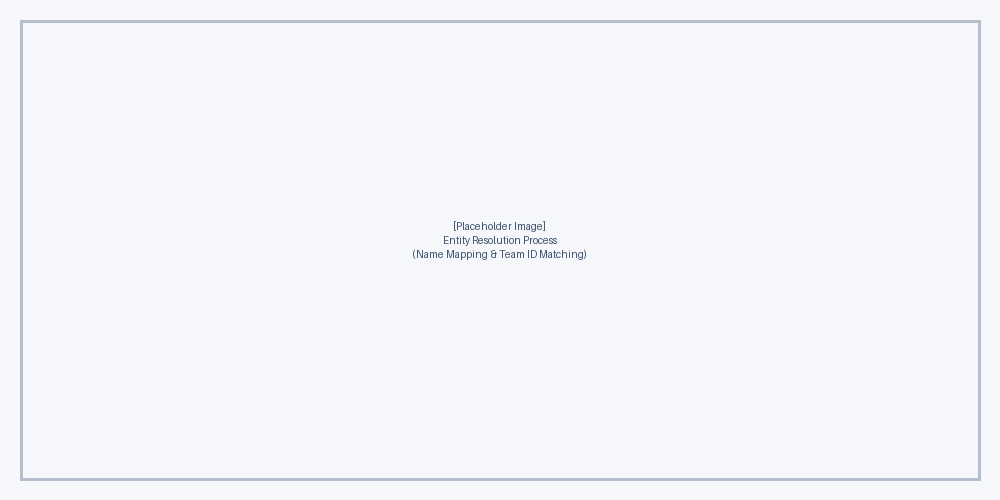
\includegraphics[width=0.75\textwidth]{images/entity_resolution.png}
    \caption{กระบวนการจับคู่และแปลงชื่อทีม (Entity Resolution) จากแหล่งข้อมูลที่แตกต่างกัน}
    \label{fig:entity_resolution}
\end{figure}

% -----------------------------------------------------------
\section{การออกแบบและพัฒนาระบบ (Pipeline \& Feature Engineering)}
% -----------------------------------------------------------

ระบบถูกออกแบบให้ทำงานเป็นสถาปัตยกรรมกระบวนการประมวลผลข้อมูลอัตโนมัติ (Automated Data Pipeline) ดังแสดงในรูปที่ \ref{fig:system_architecture} โดยแบ่งขั้นตอนการพัฒนาระบบออกเป็น 3 ส่วนหลัก

\begin{figure}[H]
    \centering
    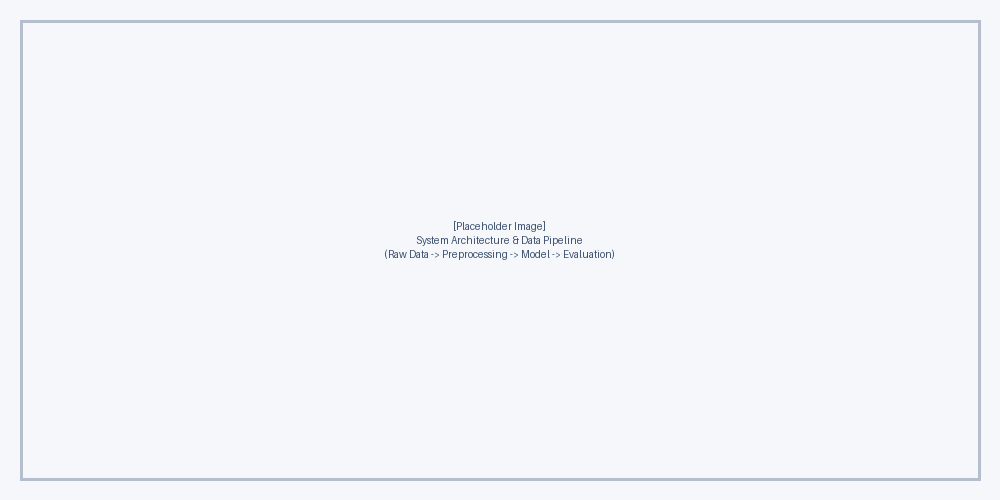
\includegraphics[width=0.85\textwidth]{images/system_architecture.png}
    \caption{ผังแสดงสถาปัตยกรรมและกระบวนการประมวลผลข้อมูล (Data Pipeline Architecture)}
    \label{fig:system_architecture}
\end{figure}

\subsection{การคำนวณคะแนน Elo Rating}
คำนวณคะแนนความแข็งแกร่งของทีมย้อนหลัง โดยปรับปรุงค่า Elo หลังจบทุกแมตช์ตามผลการแข่งขันจริงและผลต่างประตู โดยค่าความน่าจะเป็นคาดหวัง ($E_A$ และ $E_B$) และการปรับคะแนนคำนวณได้จากสมการที่ (\ref{eq:elo_expected}) และ (\ref{eq:elo_update})

\begin{equation}
    E_A = \frac{1}{1 + 10^{(R_B - R_A)/400}}
    \label{eq:elo_expected}
\end{equation}

\begin{equation}
    R'_A = R_A + K \cdot (S_A - E_A)
    \label{eq:elo_update}
\end{equation}

โดยที่ $R_A, R_B$ คือคะแนน Elo ของทีมเจ้าบ้านและทีมเยือนก่อนแข่ง, $S_A$ คือผลการแข่งจริง ($1$ เมื่อชนะ, $0.5$ เมื่อเสมอ, $0$ เมื่อแพ้) และ $K$ คือค่าพารามิเตอร์การปรับน้ำหนัก ($K=20$) ดังโค้ดตัวอย่างในรายการที่ \ref{lst:elo_code}

\begin{lstlisting}[language=Python, caption={การคำนวณและปรับปรุงคะแนน Elo Rating}, label={lst:elo_code}]
def update_elo(home_elo, away_elo, home_score, away_score, k=20):
    # คำนวณความน่าจะเป็นคาดหวัง (Expected Outcome)
    e_home = 1 / (1 + 10 ** ((away_elo - home_elo) / 400))
    e_away = 1 - e_home
    
    # กำหนดผลลัพธ์จริง (Actual Outcome)
    if home_score > away_score:
        s_home, s_away = 1.0, 0.0
    elif home_score == away_score:
        s_home, s_away = 0.5, 0.5
    else:
        s_home, s_away = 0.0, 1.0
        
    # ปรับปรุงคะแนน
    new_home_elo = home_elo + k * (s_home - e_home)
    new_away_elo = away_elo + k * (s_away - e_away)
    return new_home_elo, new_away_elo
\end{lstlisting}

\subsection{การทำ Moving Average Statistics และการป้องกัน Data Leakage}
สร้างฟีเจอร์ฟอร์มการเล่นย้อนหลัง $N$ นัด (Rolling Windows 5 และ 10 นัด) สำหรับตัวแปรประตูที่ยิงได้, ประตูที่เสีย, ค่า xG และ xGA โดยการคำนวณจะใชเฉพาะข้อมูลนัดที่ $T-1, T-2, \dots, T-N$ ก่อนวันแข่งขันจริงในนัดที่ $T$ ดังแสดงในรูปที่ \ref{fig:rolling_window} เพื่อป้องกันปัญหาข้อมูลอนาคตรั่วไหลเข้าสู่แบบจำลอง (Data Leakage)

\begin{figure}[H]
    \centering
    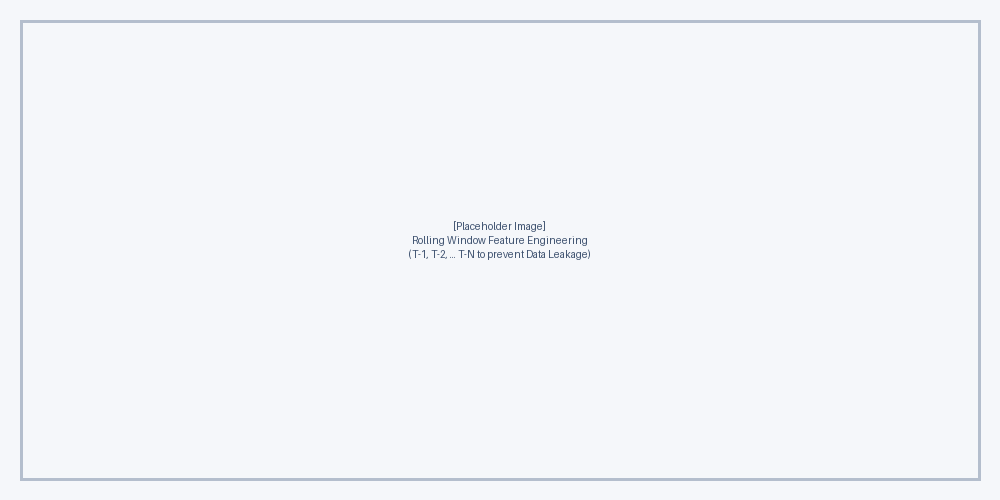
\includegraphics[width=0.8\textwidth]{images/rolling_window.png}
    \caption{แผนภาพแสดงหลักการคำนวณ Rolling Average ย้อนหลังเพื่อป้องกันปัญหา Data Leakage}
    \label{fig:rolling_window}
\end{figure}

\subsection{การแปลงราคาต่อรองเป็น Implied Probabilities}
แปลงราคาต่อรองจากเจ้ามือ (Bookmaker Odds) ให้เป็นค่าความน่าจะเป็น พร้อมปรับปรุงค่า Margin Overround เพื่อใช้เป็นฟีเจอร์อ้างอิงและ Benchmark ของแบบจำลอง

% -----------------------------------------------------------
\section{การพัฒนาแบบจำลองและการแบ่งชุดข้อมูล}
% -----------------------------------------------------------

\subsection{การแบ่งชุดข้อมูลตามลำดับเวลา (Temporal Train-Test Split)}
เนื่องจากข้อมูลการแข่งขันเป็นข้อมูลอนุกรมเวลา (Time-Series Data) การทดสอบจึงไม่สามารถใชการสุ่มแบบ K-Fold Cross Validation ปกติได้ เพราะจะทำให้ข้อมูลในอนาคตรั่วไหลไปอธิบายอดีต ผู้จัดทำจึงทำการแบ่งข้อมูลตามลำดับเวลาจริง (Temporal Split) ดังแสดงในรูปที่ \ref{fig:temporal_split}

\begin{figure}[H]
    \centering
    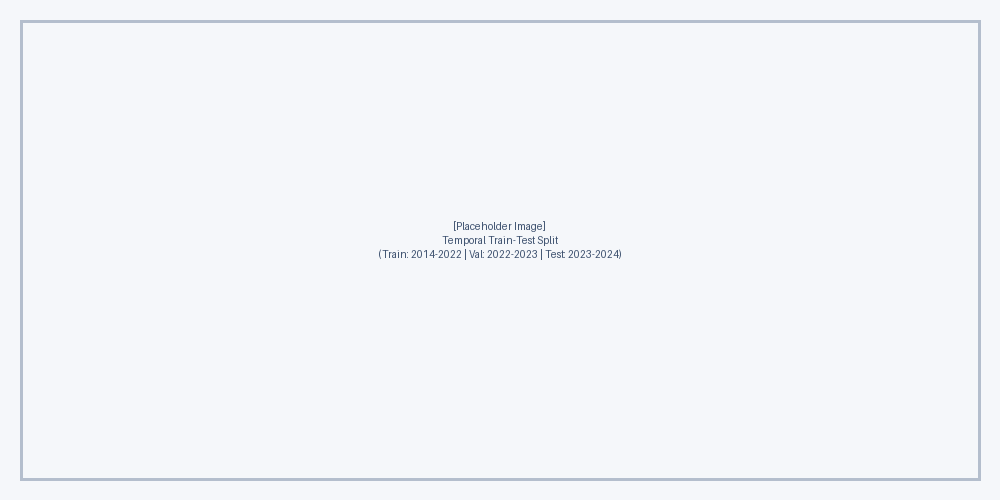
\includegraphics[width=0.85\textwidth]{images/temporal_split.png}
    \caption{การแบ่งชุดข้อมูลเพื่อการฝึกสอนและทดสอบตามลำดับเวลา (Temporal Train-Test Split)}
    \label{fig:temporal_split}
\end{figure}

รายละเอียดการแบ่งชุดข้อมูลมีดังนี้
\begin{itemize}
    \item \textbf{Train Set:} ข้อมูลฤดูกาล 2014/2015 ถึง 2021/2022 (8 ฤดูกาล รวม 3,040 แมตช์)
    \item \textbf{Validation Set:} ข้อมูลฤดูกาล 2022/2023 (1 ฤดูกาล รวม 380 แมตช์)
    \item \textbf{Test Set:} ข้อมูลฤดูกาล 2023/2024 (1 ฤดูกาล รวม 380 แมตช์)
\end{itemize}

\subsection{การเลือกและปรับแต่งแบบจำลอง (Model Selection \& Tuning)}
ผู้จัดทำได้เลือกใช้แบบจำลองทางสถิติและ Machine Learning รวม 5 แบบจำลอง ได้แก่ Logistic Regression, Random Forest, XGBoost, LightGBM และ CatBoost โดยทำการค้นหาพารามิเตอร์ที่เหมาะสมที่สุด (Hyperparameter Tuning) ผ่านกระบวนการ Grid Search และ Bayesian Optimization บน Validation Set

% -----------------------------------------------------------
\section{การทดสอบและประเมินผลระบบ (Testing \& Evaluation Framework)}
% -----------------------------------------------------------

การประเมินประสิทธิภาพของแบบจำลองบน Test Set จะวัดผลผ่านดัชนีทางสถิติที่ครอบคลุมทั้งด้านความแม่นยำและการทำนายค่าความน่าจะเป็น ดังนี้

\begin{enumerate}[label=\arabic*)]
    \item \textbf{Classification Metrics:} คำนวณค่า Accuracy, Precision, Recall และ F1-Score สำหรับผลการแข่งขันทั้ง 3 คลาส ($H, D, A$)
    \item \textbf{Multi-Class Log Loss:} วัดความแม่นยำของการประมาณค่าความน่าจะเป็น คำนวณได้จากสมการที่ (\ref{eq:logloss})
    \begin{equation}
        \text{Log Loss} = -\frac{1}{N} \sum_{i=1}^{N} \sum_{j=1}^{M} y_{ij} \log(p_{ij})
        \label{eq:logloss}
    \end{equation}
    โดยที่ $N$ คือจำนวนแมตช์ทั้งหมด ($N=380$), $M$ คือจำนวนคลาส ($M=3$), $y_{ij}$ คือค่าจริง (1 หรือ 0) และ $p_{ij}$ คือค่าความน่าจะเป็นที่แบบจำลองทำนาย
    \item \textbf{Ranked Probability Score (RPS):} คำนวณความคลาดเคลื่อนของการทำนายผลฟุตบอลที่มีลำดับสเกล \cite{hubacek2021forty}
\end{enumerate}